\section{Modificación del modelo de una universidad}

La Figura~\ref{fig:modelo-universidad} presenta la modificación propuesta por
el equipo, conservando la notación de Chen empleada en los demás diagramas.
Las líneas dobles indican participación total, las líneas simples indican
participación parcial y las flechas representan restricciones de unicidad.

\begin{figure}[htbp]
  \centering
  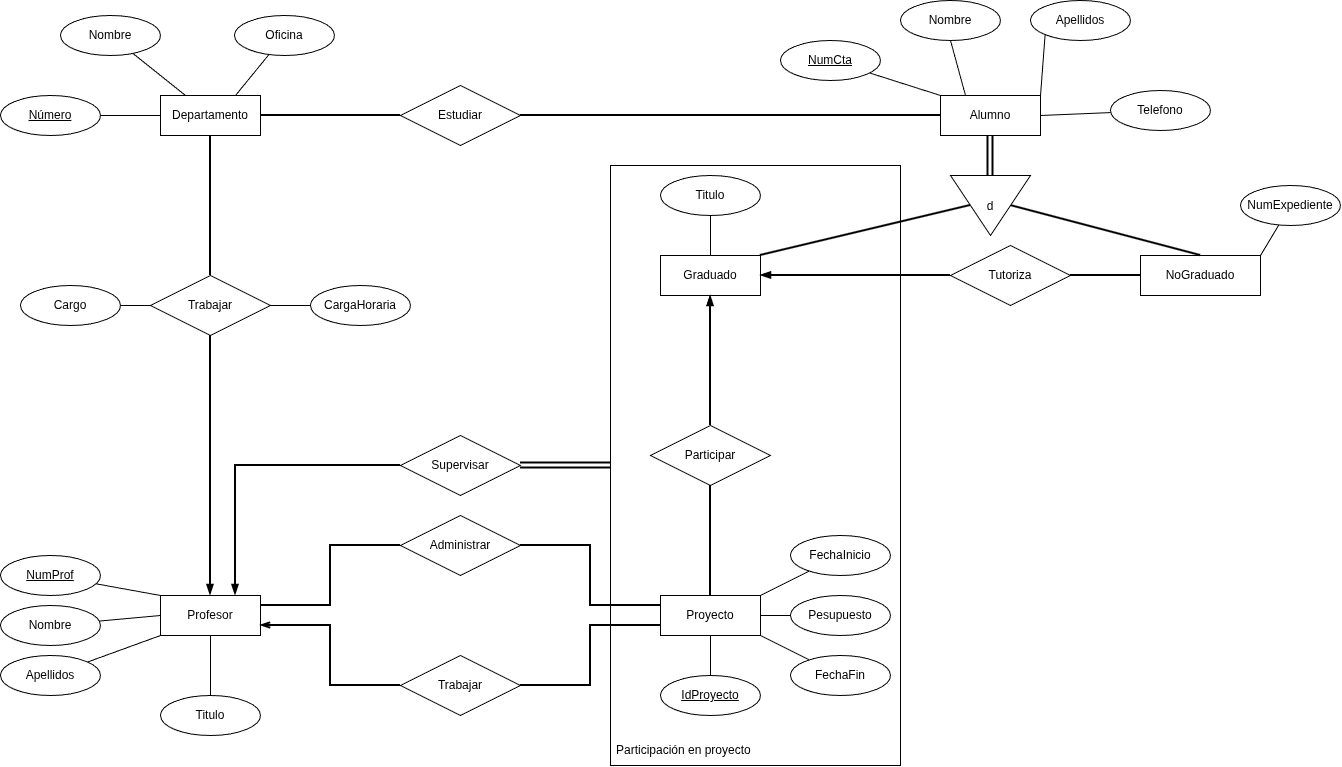
\includegraphics[width=\textwidth]{../Diagramas/Ejercicio2ii.png}
  \caption{Modelo E--R modificado para la universidad.}
  \label{fig:modelo-universidad}
\end{figure}

\subsection{Especialización de alumnos y tutoría}

\textbf{Alumno} se presenta como superentidad de \textbf{Graduado} y
\textbf{NoGraduado}. El triángulo marcado con ``d'' establece una
especialización disjunta: un alumno no puede pertenecer simultáneamente a
ambos subtipos. \textbf{Graduado} incorpora el atributo \emph{Título}, mientras
\textbf{NoGraduado} incorpora \emph{NumExpediente}.

La relación \textbf{Tutoriza} conecta ambos subtipos. La flecha dirigida hacia
\textbf{Graduado} expresa que un alumno no graduado se vincula, como máximo,
con un solo tutor; un graduado puede tutorizar a varios alumnos no graduados.
El diagrama conserva una línea simple del lado de \textbf{NoGraduado}, por lo
que su participación se representa como parcial en la propuesta gráfica.

\subsection{Cargo y carga horaria por departamento}

Los atributos \emph{Cargo} y \emph{CargaHoraria} se colocan en la relación
\textbf{Trabajar} entre \textbf{Departamento} y \textbf{Profesor}. Esta
ubicación indica que sus valores describen la asignación de un profesor dentro
de un departamento y no al profesor o al departamento de forma aislada. La
flecha incluida en la propuesta representa la restricción de unicidad elegida
por el equipo para impedir la repetición de un cargo dentro del mismo
departamento.

\subsection{Participación en proyectos y supervisión}

\textbf{Graduado} participa en \textbf{Proyecto} mediante la relación
\textbf{Participar}. El recuadro que agrupa ambas entidades y su relación
constituye la agregación \emph{Participación en proyecto}. Esta agregación se
relaciona con \textbf{Profesor} mediante \textbf{Supervisar}, lo que permite
asignar un profesor a cada participación concreta de un alumno graduado en un
proyecto. La línea doble entre la agregación y \textbf{Supervisar} expresa la
participación total mostrada en el diagrama.

Las relaciones \textbf{Administrar}, \textbf{Estudiar} y las demás estructuras
del modelo original se conservan sin alteraciones, pues el enunciado no solicita
modificarlas.
